\Aufgabe[Bisimulation \& Simulation Relations\hfill\textbf{(1 Point)}]

Consider the following Kripke structures $K_1$ and $K_2$ and the bisimulation relation $$H = \{ (s_0, t_0), (s_1, t_1), (s_2, t_2), (s_3, t_3), (s_4, t_4), (s_5, t_5), $$
$$(s_6, t_6), (s_6, t_7), (s_7, t_8), (s_8, t_9), (s_9, t_{10}) \}.$$

\begin{center}
\begin{minipage}{0.48\textwidth}
	\scalebox{0.8}{
  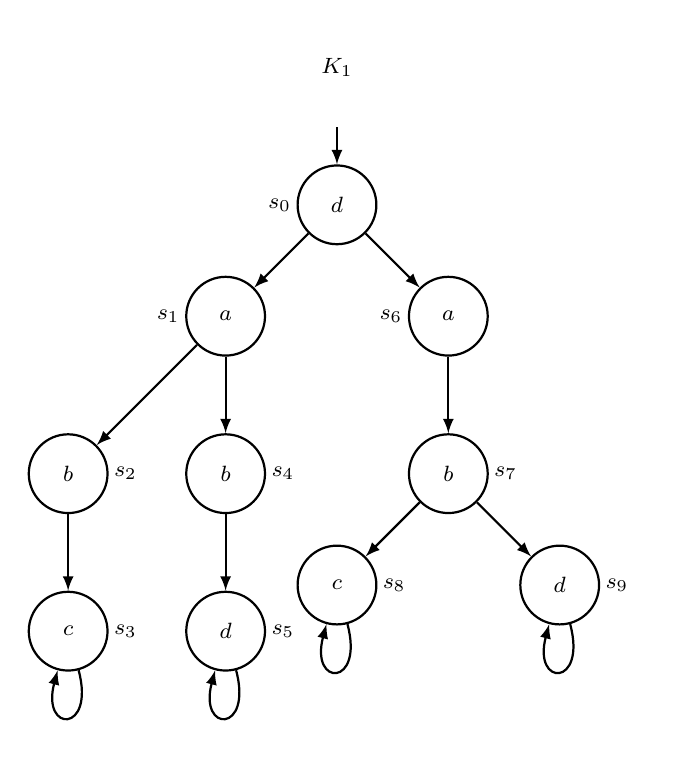
\begin{tikzpicture}[->,scale=1,label distance=-3mm,>= latex, node distance = 2cm]
    \tikzstyle{every node}=[shape=circle,minimum size=10mm,font=\footnotesize];
    \tikzstyle{every path} = [draw,thick];
    
    \node[draw] (n0) [label=left:$s_0$] {$d$};
    
    \node (tmp) [above of=n0, node distance=1.5cm] {};
    \node (tmp2) [above of=tmp,node distance=0.25cm] {$K_1$};
    
    \node[draw] (n6) [below right of=n0,label=left:$s_6$] {$a$};
    \node[draw] (n1) [below left of=n0,label=left:$s_1$] {$a$};
    \node[draw] (n4) [below of=n1,label=right:$s_4$] {$b$};
    \node[draw] (n2) [left of=n4,label=right:$s_2$] {$b$};
    \node[draw] (n3) [below of=n2,label=right:$s_3$] {$c$};
    \node[draw] (n5) [below of=n4,label=right:$s_5$] {$d$};
    \node[draw] (n8) [below of=n6,label=right:$s_7$] {$b$};
    \node[draw] (n9) [below left of=n8,label=right:$s_8$] {$c$};
    \node[draw] (n10) [below right of=n8,label=right:$s_{9}$] {$d$};
    
    \draw[->] (tmp) -- (n0);
    \draw[->] (n0) -- (n1);
    \draw[->] (n0) -- (n6);
    \draw[->] (n1) -- (n2);
    \draw[->] (n1) -- (n4);
    \draw[->] (n2) -- (n3);
    \draw[->] (n4) -- (n5);
		\draw[->] (n6) -- (n8);
		\draw[->] (n8) -- (n9);
		\draw[->] (n8) -- (n10);
		    
    \path[loop below] (n3) to (n3);
    \path[loop below] (n5) to (n5);
    \path[loop below] (n9) to (n9);
    \path[loop below] (n10) to (n10);
    
\end{tikzpicture}
}
\end{minipage}
\hfill
\begin{minipage}{0.48\textwidth}
	\scalebox{0.8}{
  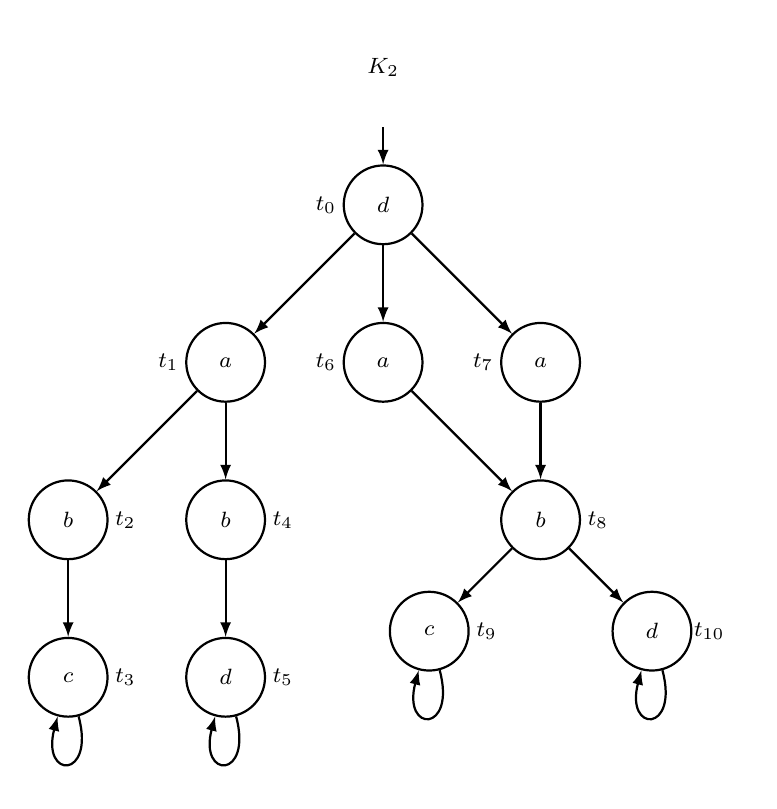
\begin{tikzpicture}[->,scale=1,label distance=-3mm,>= latex, node distance = 2cm]
    \tikzstyle{every node}=[shape=circle,minimum size=10mm,font=\footnotesize];
    \tikzstyle{every path} = [draw,thick];
    
    \node[draw] (n0) [label=left:$t_0$] {$d$};
    
    \node (tmp) [above of=n0, node distance=1.5cm] {};
    \node (tmp2) [above of=tmp,node distance=0.25cm] {$K_2$};
    
    \node[draw] (n6) [below of=n0,label=left:$t_6$] {$a$};
    \node[draw] (n1) [left of=n6,label=left:$t_1$] {$a$};
    \node[draw] (n7) [right of=n6,label=left:$t_7$] {$a$};
    \node[draw] (n4) [below of=n1,label=right:$t_4$] {$b$};
    \node[draw] (n2) [left of=n4,label=right:$t_2$] {$b$};
    \node[draw] (n3) [below of=n2,label=right:$t_3$] {$c$};
    \node[draw] (n5) [below of=n4,label=right:$t_5$] {$d$};
    \node[draw] (n8) [below of=n7,label=right:$t_8$] {$b$};
    \node[draw] (n9) [below left of=n8,label=right:$t_9$] {$c$};
    \node[draw] (n10) [below right of=n8,label=right:$t_{10}$] {$d$};
    
    \draw[->] (tmp) -- (n0);
    \draw[->] (n0) -- (n1);
    \draw[->] (n0) -- (n6);
    \draw[->] (n0) -- (n7);
    \draw[->] (n1) -- (n2);
    \draw[->] (n1) -- (n4);
    \draw[->] (n2) -- (n3);
    \draw[->] (n4) -- (n5);
		\draw[->] (n6) -- (n8);
		\draw[->] (n7) -- (n8);
		\draw[->] (n8) -- (n9);
		\draw[->] (n8) -- (n10);
		    
    \path[loop below] (n3) to (n3);
    \path[loop below] (n5) to (n5);
    \path[loop below] (n9) to (n9);
    \path[loop below] (n10) to (n10);
    
\end{tikzpicture}
}
\end{minipage}
\end{center}


\paragraph{a)} Give a simulation relation $H'$ such that $K_1 \leq K_2$ and $|H'| < |H|$.\hfill\textbf{(0.5 Points)}

$$H' = \{ (s_0, t_0), (s_1, t_1), (s_2, t_2), (s_3, t_3), (s_4, t_4), (s_5, t_5), $$
$$(s_6, t_7), (s_7, t_8), (s_8, t_9), (s_9, t_{10}) \}.$$

$|H'| = 10$

\paragraph{b)} Give a simulation relation $H''$ such that $K_1 \leq K_2$ and $|H''| > |H|$.\hfill\textbf{(0.5 Points)}

$$H'' = \{ (s_0, t_0), (s_1, t_1), (s_2, t_2), (s_3, t_3), (s_4, t_4), (s_5, t_5), $$
$$(s_6, t_6), (s_6, t_7), (s_7, t_8), (s_8, t_9), (s_9, t_{10}), (s_2,t_8), (s_4, t_8) \}.$$

$|H''| = 13$
